\documentclass[11pt]{article}

%  USE PACKAGES  ---------------------- 
\usepackage[margin=0.75in,vmargin=1in]{geometry}
\usepackage{amsmath,amsthm,amsfonts}
\usepackage{amssymb}
\usepackage{fancyhdr}
\usepackage{enumerate}
\usepackage{mathtools}
\usepackage{hyperref,color}
\usepackage{enumitem,amssymb}
\usepackage{graphicx}
\newcommand\tab[1][1cm]{\hspace*{#1}}
\newlist{todolist}{itemize}{4}
\setlist[todolist]{label=$\square$}
\usepackage{pifont}
\newcommand{\cmark}{\ding{51}}%
\newcommand{\xmark}{\ding{55}}%
\newcommand{\done}{\rlap{$\square$}{\raisebox{2pt}{\large\hspace{1pt}\cmark}}%
\hspace{-2.5pt}}
\newcommand{\HREF}[2]{\href{#1}{#2}}
\usepackage{textcomp}
\usepackage{listings}
\lstset{
basicstyle=\small\ttfamily,
% columns=flexible,
upquote=true,
breaklines=true,
showstringspaces=false
}
\usepackage{longtable}
\usepackage{subcaption}
\usepackage{blindtext}
\usepackage{titlesec}
%  -------------------------------------------- 

%  HEADER AND FOOTER (DO NOT EDIT) ----------------------
\newcommand{\problemnumber}{0}
\pagestyle{fancy}
\fancyhead{}
% \fancyhead[L]{\textbf{\problemnumber}}
\newcommand{\newquestion}[1]{
\clearpage % page break and flush floats
\renewcommand{\problemnumber}{#1} % set problem number for header
\phantom{}  % Put something on the page so it shows
}
\fancyfoot[L]{IE 332}
\fancyfoot[C]{Project submission}
\fancyfoot[R]{Page \thepage}
\renewcommand{\footrulewidth}{0.4pt}

%  --------------------------------------------


%  COVER SHEET (FILL IN THE TABLE AS INSTRUCTED IN THE ASSIGNMENT) ----------------------
\newcommand{\addcoversheet}{
\clearpage
\thispagestyle{empty}
\vspace*{0.5in}

\begin{center}
\Huge{{\bf IE332 Project \#2}} % <-- replace with correct assignment #

Due: April 28th, 11:59pm EST % <-- replace with correct due date and time
\end{center}

\vspace{0.3in}

\noindent We have {\bf read and understood the assignment instructions}. We certify that the submitted work does not violate any academic misconduct rules, and that it is solely our own work. By listing our names below we acknowledge that any misconduct will result in appropriate consequences. 

\vspace{0.2in}

\noindent {\em ``As a Boilermaker pursuing academic excellence, I pledge to be honest and true in all that I do.
Accountable together -- we are Purdue.''}

\vspace{0.3in}

\begin{table}[h!]
  \begin{center}
    \label{tab:table1}
    \begin{tabular}{c|ccccc|c|c}
      Student & Q1 & Q2 & Q3 & Q4 & Q5 & Overall & DIFF\\
      \hline
      Taylor Kalata & 0 & 0 & 0 & 0 & 0 & 0 & 0\\
      Alex Hart & 0 & 0 & 0 & 0 & 0 & 0 & 0\\
      Grant Laneve & 0 & 0 & 0 & 0 & 0 & 0 & 0\\
      Angelica Jovceski & 0 & 0 & 0 & 0 & 0 & 0 & 0\\
      Sam Preston & 0 & 0 & 0 & 0 & 0 & 0 & 0\\
      \hline
      St Dev & 0 & 0 & 0 & 0 & 0 & 0 & 0
    \end{tabular}
  \end{center}
\end{table}

\vspace{0.2in}

\noindent Date: \today.
}


%  -----------------------------------------

\begin{document}

\addcoversheet
\newpage
\tableofcontents


% BEGIN YOUR ASSIGNMENT HERE:
\newpage
\section{Introduction}
%Overview of the project and the required algorithms
%angelica

Machine learning enables the development of complex models to learn from data and perform various tasks such as image classification. Image classification is where a model learns to recognize and categorize images into different classes. Although, with any technology, machine learning algorithms are not immune to attacks.

Adversarial attacks have been developed to fool machine learning models by making small, changes to the input data, which cause the model to incorrectly classify the image. Adversarial attacks can be used to test the robustness of machine learning models and can also be used to deceive and manipulate models in the real world. 

In this project, we aimed to train a voting-based optimization algorithm to perform adversarial attacks on a binary image classifier. We used five different machine learning algorithms to fool the classifier, and placed them within another algorithm that assigns weights to them based on their expected performance given the image.


The ultimate goal of this project was to successfully fool the provided image classifier with a given pixel budget and to do so in less than 10 seconds per image. We evaluated our models on a set of reserved 100\% accurate data and scored them based on their successful fooled images at different budget levels. Our report will detail the rationale for selecting each of the five machine learning algorithms, how we trained them, how our optimizer allocates the votes, and why such an approach should work. We will also provide an analysis of the performance of our algorithms, their accuracy, runtime complexity, and average wall-time, as well as the lessons learned and future directions for research in this area.





\section{Purpose of Image Classifiers}
%applications of image classifiers and why they benefit different industries
%alex
In the age of Artificial Intelligence and the Internet of Things, image classifiers play an important role in providing analysis for the massive amounts of unstructured image data we obtain. Image classification is the basis for computer vision: a field in which the goal is to enable a computer to see and understand objects in photos and videos. In some cases of classification, computers access massive amounts of data and can sense details leading to a high level of accuracy in classification that can far exceed that of a human (“What is …”, 2023). 
While in this project the model is distinguishing between only grass and dandelions with a given data set, search engines such as Google are given less constraints and more data to decipher in order to predict images based on random keywords or identify objects in a reverse image search. Visual search engines are one of many applications of image classifiers. Some other prevalent examples include facial recognition, traffic control systems, and self-driving cars (Boesch, 2023).


\section{Danger of Adversary Attacks}
%explain why these attacks can be dangerous
%taylor
As mentioned above, image classifiers can be a helpful technological advance in a variety of industries. However, these classifier models can be very susceptible to adversarial attacks due to their brittle nature (PureAI Editors, 2021). Slightly changing pixels of images can completely change the model result. A simple binary image classifier to detect a dandelion will probably not be a target of an attack in the real world. But when we look at industries like medical, military, financial, security, etc, the effects of a faulty model can have serious consequences. Not only can these attacks cause incorrect classification but also doing so with reported high confidence in its prediction. For example, adversary attacks can be very dangerous with the emerging presence of self-driving cars. The "sight" of the car is made possible through deep neural networks that make up the model to classify different objects the car encounters. When the model is under attack, it can cause images to be classified incorrectly leading to accidents and injury. The self-driving car may identify a stop sign as a speed limit sign; graffiti could be identified as a person or animal in the road; another car could be mistaken for an open road. These are just some of many ways an adversary attack could potentially harm humans. It can especially be dangerous due to the fact the humans do not see any potential threat. If people are not aware of these possible attacks and their implications, it is easy to trust the models and not think twice about incorrect classifications. 
\begin{figure}[h]
\begin{center}
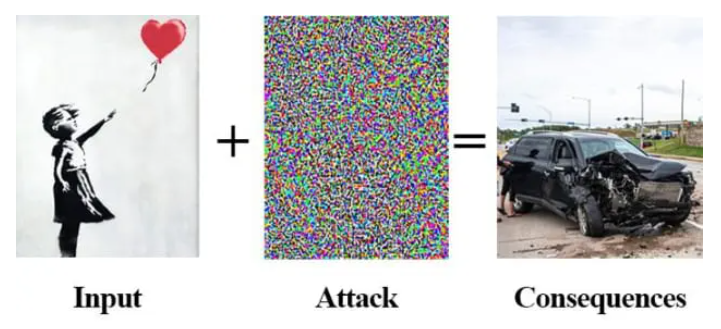
\includegraphics[width=0.75\textwidth, height=5cm]{car_accident.png}
\caption{Adversarial Attack Effect}
\label{fig:figure2}
\end{center}
\end{figure}

Because of the potential danger in many industries, defense against these attacks is being researched heavily (Wiggers, 2021). One way involves modifying a model to respond to input triggers that are used in these attacks. Researchers are implementing a Trojan horse method to test the effectiveness of their defense tactics. This allows them to better understand how the model reacts to attacks and what modifications will benefit the robustness of the neural networks. This method provides a basis for further research and techniques to boost model security. Increasing the reliability of these image classifiers will allow different fields to safely implement them to elevate the ability of machines in industry practice.

\section{Algorithm explanations}
%explain each algorithm goal/how it works

%need to ask Lucas how to interpret the results of running the test loop
%occlude function does not trick or lower accuracy as of now
%blurry function does not trick but lowers accuracy
%add noise function does not trick but lowers accuracy (have ti add isoblur to it though)
%color function drastically lowers accuracy percentage for dandelion pictures but not grass

\section{Efficiency trade-off}
%general discussion of efficiency vs quality inverse relationship
% Grant



    
\newpage
\section{References}
\begin{verbatim}
Editors01/05/2021, P. A. I. (n.d.). Defending machine learning image classification modelsfrom attacks. Pure AI. Retrieved April 23, 2023, from 
https://pureai.com/articles/2021/01/05/defending-model-attacks.aspx#:~:text=However%2C%20it%20has%20been%20known%20for%20several%20years,the%20image%20is%20completely%20misclassified%20by%20the%20model.   

Wiggers, K. (2021, May 29). Adversarial attacks in machine learning: What they are and how to stop them. VentureBeat. Retrieved April 23, 2023, from https://venturebeat.com/security/adversarial-attacks-in-machine-learning-what-they-are-and-how-to-stop-them/ 

Boesch, G. (2023, February 24). A complete guide to Image Classification in 2023. viso.ai. Retrieved April 24, 2023, from https://viso.ai/computer-vision/image-classification/#:~:text=Image%20Classification%20is%20the%20Basis%20of%20Computer%20Vision,-The%20field%20of&text=It%20forms%20the%20basis%20for,%2C%20machine%20vision%2C%20and%20more. 

What is Computer Vision? Microsoft Azure. (2023). Retrieved April 24, 2023, from https://azure.microsoft.com/en-us/resources/cloud-computing-dictionary/what-is-computer-vision/#:~:text=Computer%20vision%20is%20a%20field,tasks%20that%20replicate%20human%20capabilities. 
\end{verbatim}

\begin{thebibliography}{4}

\end{thebibliography}

\section{Appendix}
\subsection{Testing/Correctness/Verification}
%correctness proofs of loops
%results of algorithms

\subsection{Runtime complexity/Walltime}
%explanation of how to calculate runtime
%runtime for each algorithm
%walltime is actual time it takes to run, explain difference
%sam
To calculate runtime for an algorithm, we first identify the number of operations for each iteration of the algorithm. These operations can be arithmetic operations, comparisons, and assignment operations. We represent these as weights. Next, we determine a mathematical expression in relation to the input size, n.
We then combine the weights, or number of operations, and multiply that by the mathematical expression that represents the time complexity.
\newline \newline Walltime is a term that represents the real-time of an algorithm, in a linear sense. Start to stop, for simpler terms. Runtime, on the other hand, refers to the time it takes to execute the code or instructions, excluding the idle and/or waiting time. 

\subsection{Performance}
%before and after pictures




\subsection{Algorithm Justification}
%why we selected each algorithm 
%what the weightings would be when combined into 1 algorithm

%\begin{figure}[h]
%\centering
%\subfigure[Figure 1: Label 1]{\includegraphics[width=0.4\linewidth]{picture_1.png}}
%\subfigure[Figure 2: Label 2]{\includegraphics[width=0.4\linewidth]{picture_2.png}}
%\end{figure}

\end{document}
